\documentclass{standalone}
\usepackage{tikz}
\usetikzlibrary{patterns, positioning}
\usepackage[sfdefault]{ClearSans} %% option 'sfdefault' activates Clear Sans as the default text font
\usepackage[T1]{fontenc}

\begin{document}
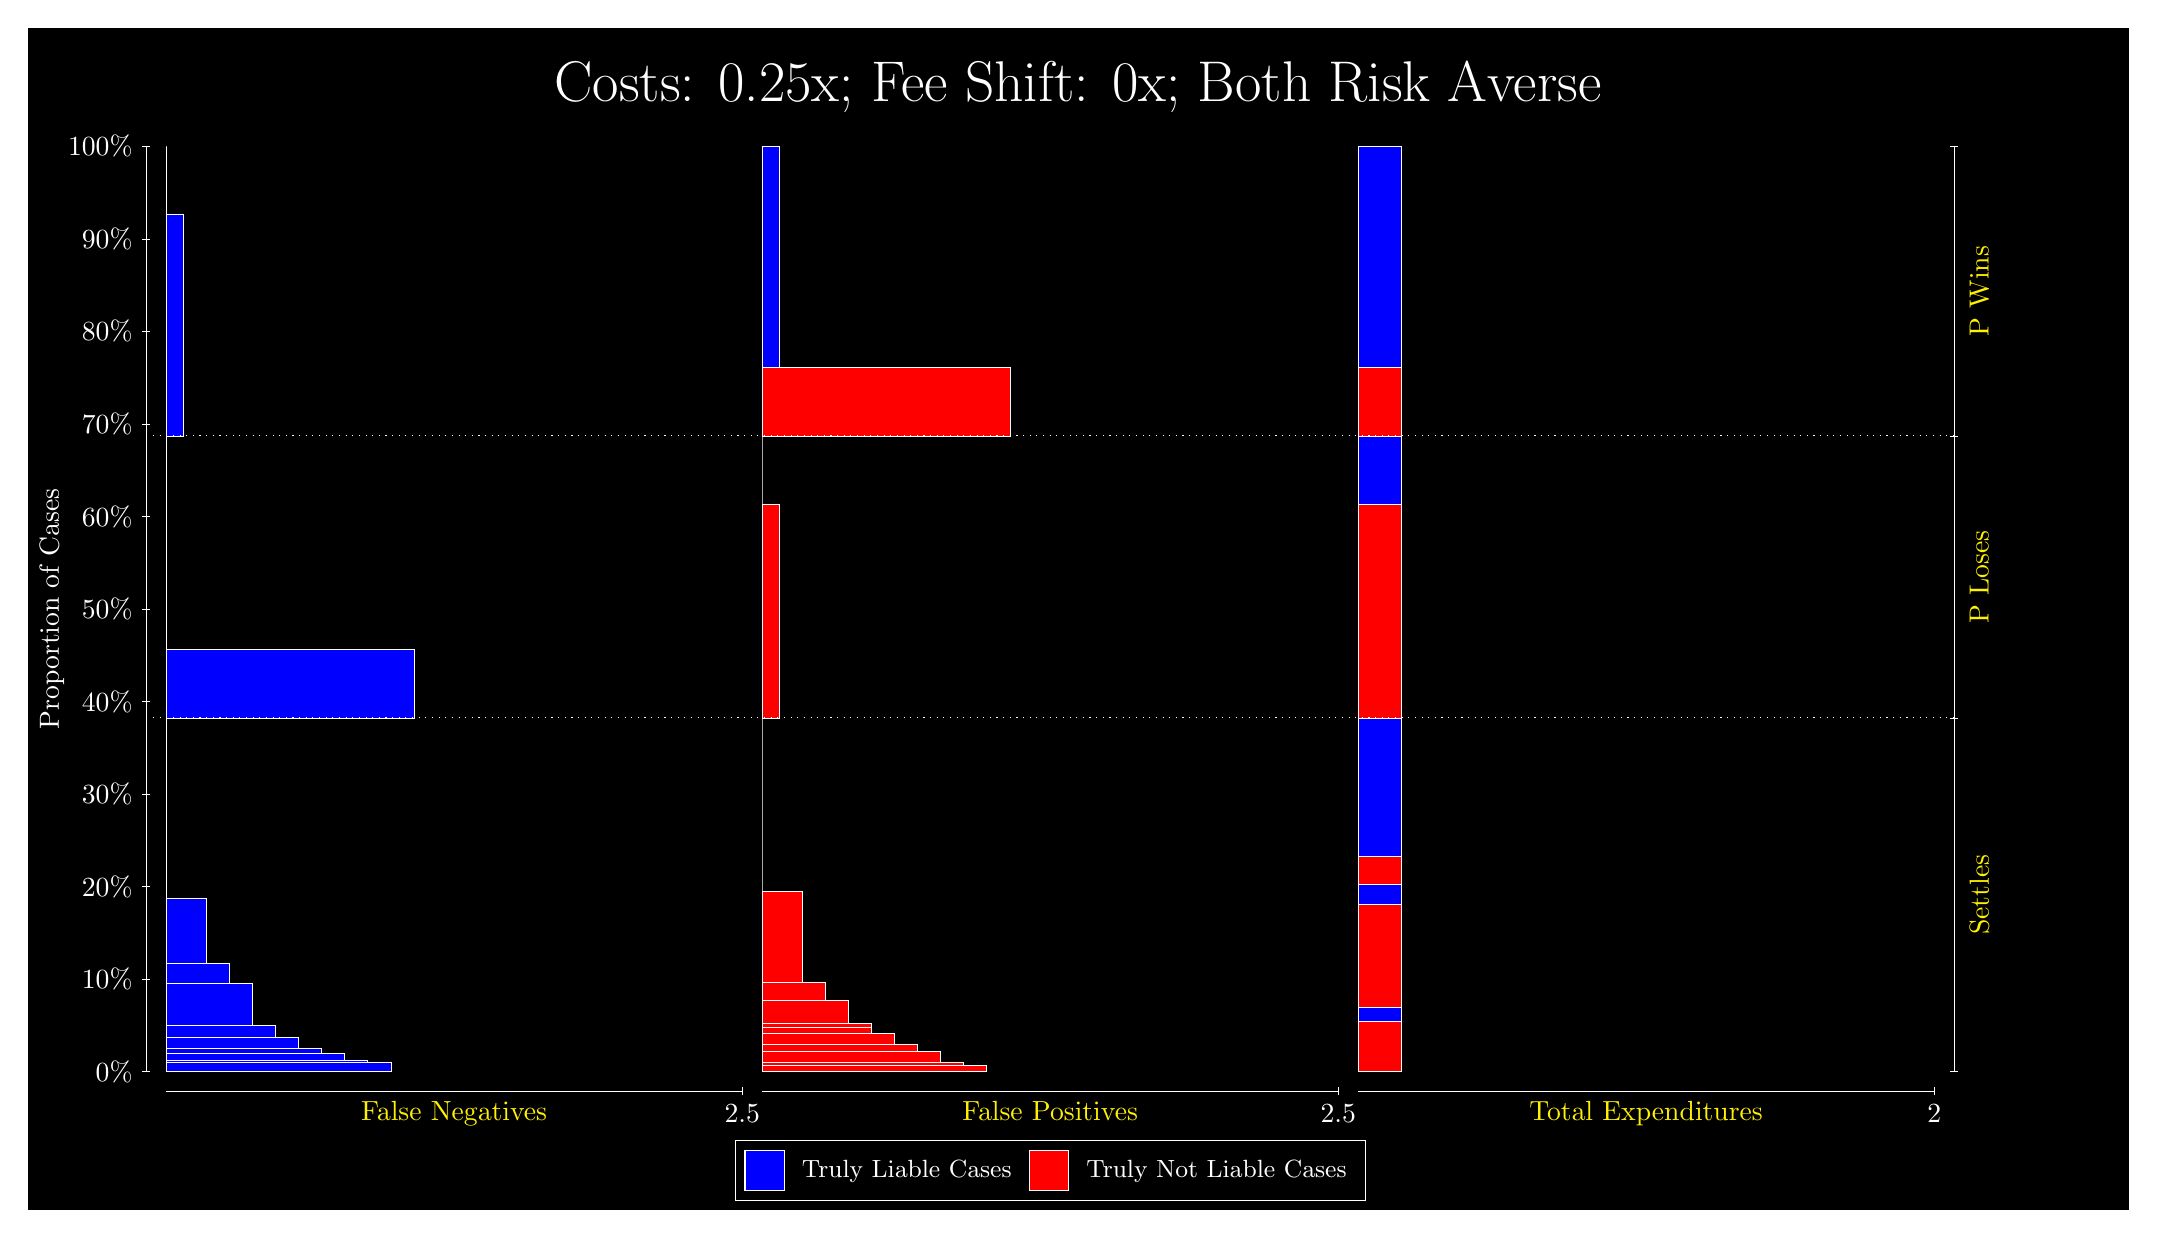
\begin{tikzpicture}
\draw[fill=black] (0,0) rectangle (26.667,15);
\draw[text=white] (0,13.5) rectangle (26.667,15) node[midway] {\huge Costs: 0.25x; Fee Shift: 0x; Both Risk Averse};
\draw[white, very thin] (1.5,1.75) -- (1.5,13.5);
\node[rotate=90, text=white, anchor=center] at (0.3, 7.625) {Proportion of Cases};
\draw[white, very thin] (1.45,1.75) -- (1.55,1.75);
\node[text=white, anchor=east] at (1.45, 1.75) {0\%};
\draw[white, very thin] (1.45,2.925) -- (1.55,2.925);
\node[text=white, anchor=east] at (1.45, 2.925) {10\%};
\draw[white, very thin] (1.45,4.1) -- (1.55,4.1);
\node[text=white, anchor=east] at (1.45, 4.1) {20\%};
\draw[white, very thin] (1.45,5.275) -- (1.55,5.275);
\node[text=white, anchor=east] at (1.45, 5.275) {30\%};
\draw[white, very thin] (1.45,6.45) -- (1.55,6.45);
\node[text=white, anchor=east] at (1.45, 6.45) {40\%};
\draw[white, very thin] (1.45,7.625) -- (1.55,7.625);
\node[text=white, anchor=east] at (1.45, 7.625) {50\%};
\draw[white, very thin] (1.45,8.8) -- (1.55,8.8);
\node[text=white, anchor=east] at (1.45, 8.8) {60\%};
\draw[white, very thin] (1.45,9.975) -- (1.55,9.975);
\node[text=white, anchor=east] at (1.45, 9.975) {70\%};
\draw[white, very thin] (1.45,11.15) -- (1.55,11.15);
\node[text=white, anchor=east] at (1.45, 11.15) {80\%};
\draw[white, very thin] (1.45,12.325) -- (1.55,12.325);
\node[text=white, anchor=east] at (1.45, 12.325) {90\%};
\draw[white, very thin] (1.45,13.5) -- (1.55,13.5);
\node[text=white, anchor=east] at (1.45, 13.5) {100\%};

\draw[white, very thin] (24.457,1.75) -- (24.457,13.5);
\draw[white, very thin] (24.407,1.75) -- (24.507,1.75);
\node[anchor=west] at (24.407, 1.75) {};
\draw[white, very thin] (24.407,6.2419) -- (24.507,6.2419);
\node[anchor=west] at (24.407, 6.2419) {};
\draw[white, very thin] (24.407,9.8231) -- (24.507,9.8231);
\node[anchor=west] at (24.407, 9.8231) {};
\draw[white, very thin] (24.407,13.5) -- (24.507,13.5);
\node[anchor=west] at (24.407, 13.5) {};

\draw[white, very thin, fill=blue] (1.75,1.75) rectangle (4.6044,1.8633);
\draw[white, very thin, fill=blue] (1.75,1.8633) rectangle (4.3116,1.897);
\draw[white, very thin, fill=blue] (1.75,1.897) rectangle (4.0188,1.9835);
\draw[white, very thin, fill=blue] (1.75,1.9835) rectangle (3.7261,2.0468);
\draw[white, very thin, fill=blue] (1.75,2.0468) rectangle (3.4333,2.1878);
\draw[white, very thin, fill=blue] (1.75,2.1878) rectangle (3.1406,2.3404);
\draw[white, very thin, fill=blue] (1.75,2.3404) rectangle (2.8478,2.8645);
\draw[white, very thin, fill=blue] (1.75,2.8645) rectangle (2.5551,3.1204);
\draw[white, very thin, fill=blue] (1.75,3.1204) rectangle (2.2623,3.9488);
\draw[white, very thin, fill=red] (1.75,3.9488) rectangle (1.75,6.2419);
\draw[white, very thin, fill=blue] (1.75,6.2419) rectangle (4.8971,7.1078);
\draw[white, very thin, fill=red] (1.75,7.1078) rectangle (1.75,9.8231);
\draw[white, very thin, fill=blue] (1.75,9.8231) rectangle (1.9696,12.633);
\draw[white, very thin, fill=red] (1.75,12.633) rectangle (1.75,13.5);
\draw[white, very thin, fill=red] (9.3189,1.75) rectangle (12.173,1.8298);
\draw[white, very thin, fill=red] (9.3189,1.8298) rectangle (11.88,1.8679);
\draw[white, very thin, fill=red] (9.3189,1.8679) rectangle (11.588,2.012);
\draw[white, very thin, fill=red] (9.3189,2.012) rectangle (11.295,2.0969);
\draw[white, very thin, fill=red] (9.3189,2.0969) rectangle (11.002,2.2405);
\draw[white, very thin, fill=red] (9.3189,2.2405) rectangle (10.709,2.3137);
\draw[white, very thin, fill=red] (9.3189,2.3137) rectangle (10.709,2.3682);
\draw[white, very thin, fill=red] (9.3189,2.3682) rectangle (10.417,2.6576);
\draw[white, very thin, fill=red] (9.3189,2.6576) rectangle (10.124,2.8777);
\draw[white, very thin, fill=red] (9.3189,2.8777) rectangle (9.8312,4.043);
\draw[white, very thin, fill=blue] (9.3189,4.043) rectangle (9.3189,6.2419);
\draw[white, very thin, fill=red] (9.3189,6.2419) rectangle (9.5384,8.9572);
\draw[white, very thin, fill=blue] (9.3189,8.9572) rectangle (9.3189,9.8231);
\draw[white, very thin, fill=red] (9.3189,9.8231) rectangle (12.466,10.69);
\draw[white, very thin, fill=blue] (9.3189,10.69) rectangle (9.5384,13.5);
\draw[white, very thin, fill=red] (16.888,1.75) rectangle (17.437,2.3872);
\draw[white, very thin, fill=blue] (16.888,2.3872) rectangle (17.437,2.5707);
\draw[white, very thin, fill=red] (16.888,2.5707) rectangle (17.437,3.8797);
\draw[white, very thin, fill=blue] (16.888,3.8797) rectangle (17.437,4.134);
\draw[white, very thin, fill=red] (16.888,4.134) rectangle (17.437,4.4809);
\draw[white, very thin, fill=blue] (16.888,4.4809) rectangle (17.437,6.2419);
\draw[white, very thin, fill=red] (16.888,6.2419) rectangle (17.437,8.9572);
\draw[white, very thin, fill=blue] (16.888,8.9572) rectangle (17.437,9.8231);
\draw[white, very thin, fill=red] (16.888,9.8231) rectangle (17.437,10.69);
\draw[white, very thin, fill=blue] (16.888,10.69) rectangle (17.437,13.5);
\draw[white, dotted] (1.5,6.2419) -- (24.457,6.2419);
\draw[white, dotted] (1.5,9.8231) -- (24.457,9.8231);
\draw[white, very thin] (1.75,1.5) -- (9.0689,1.5);
\node[text=yellow, anchor=north] at (5.4094, 1.5) {False Negatives};
\draw[white, very thin] (9.0689,1.45) -- (9.0689,1.55);
\node[text=white, anchor=north] at (9.0689, 1.45) {2.5};

\draw[white, very thin] (9.3189,1.5) -- (16.638,1.5);
\node[text=yellow, anchor=north] at (12.978, 1.5) {False Positives};
\draw[white, very thin] (16.638,1.45) -- (16.638,1.55);
\node[text=white, anchor=north] at (16.638, 1.45) {2.5};

\draw[white, very thin] (16.888,1.5) -- (24.207,1.5);
\node[text=yellow, anchor=north] at (20.547, 1.5) {Total Expenditures};
\draw[white, very thin] (24.207,1.45) -- (24.207,1.55);
\node[text=white, anchor=north] at (24.207, 1.45) {2};

\node[text=yellow, centered, rotate=90] at (24.777, 3.9959) {Settles};
\node[text=yellow, centered, rotate=90] at (24.777, 8.0325) {P Loses};
\node[text=yellow, centered, rotate=90] at (24.777, 11.662) {P Wins};

\draw (12.978300999999998,1.5) node[draw=none] (baseCoordinate) {};
\begin{scope}[align=center]
        \matrix[scale=0.5, draw=white, below=0.5cm of baseCoordinate, nodes={draw}, column sep=0.1cm]{
            \node[rectangle, draw, minimum width=0.5cm, minimum height=0.5cm, fill=blue] {}; &
            \node[draw=none, font=\small, text=white] (B) {Truly Liable Cases}; &
            \node[rectangle, draw, minimum width=0.5cm, minimum height=0.5cm, fill=red] {}; &
            \node[draw=none, font=\small, text=white] (B) {Truly Not Liable Cases}; \\
            };
\end{scope}

\end{tikzpicture}
\end{document}